\section{Traits Classes\label{arr_sec:traits}}
%=======================

As mentioned in the introduction of this chapter, the traits class
encapsulates the definitions of the geometric entities and
implements the geometric predicates and constructions needed by
the \ccc{Arrangement_2} class and by its peripheral algorithms. We also
mention throughout the chapter that there are different levels of
requirements from the traits class, namely the traits class can model
different concept refinement-levels.

%--------------------------------------------------
\subsection{The Hierarchy of Traits-Class Concepts
\label{arr_sssec:tr_concepts}}
%--------------------------------------------------

\subsubsection{The Basic Concept
\label{arr_sssec:tr_basic_concept}}
%~~~~~~~~~~~~~~~~~~~~~~~~~~~~~~~~~~

A model of the basic concept, \ccc{ArrangementBasicTraits_2},
needs to define the types \ccc{Point_2} and
\ccc{X_monotone_curve_2}, where objects of the first type are
the geometric mapping of arrangement vertices, and objects of the
latter type are the geometric mapping of edges. Such a model has to
support in addition the following set of operations: 
\begin{description}
\item[\ccc{Compare_x_2}:] Compares the $x$-coordinates of two points.
  %
\item[\ccc{Compare_xy_2}:] Compares two points lexicographically, by
  their $x$-coordinates and then (in case of equality) by their
  $y$-coordinates.
  %
\item[\ccc{Construct_min_vertex_2},\ccc{Construct_max_vertex_2}:]
  Returns the left endpoint (similarly, the right endpoint) of
  an $x$-monotone curve.
  %
\item[\ccc{Compare_y_at_x_2}:] Given an $x$-monotone curve $c$ and a
  point $p$ that lies in its $x$-range, this predicate determines
  whether $p$ lies below, above or on $c$.
  %
\item[\ccc{Compare_y_at_x_right_2}:]
  Given two $x$-monotone curves $c_1$ and $c_2$ that share a common
  left endpoint $p$, this predicate determines whether $c_1$ lies
  above or under $c_2$ immediately to the right of $p$, or whether the
  two curves coincide there.
\item[\ccc{Equal_2}:] Checks two points and two curves for equality
  (two curves are equal if their graph is the same).
  %
\item[\ccc{Is_vertical_2}:]
  Determines whether an $x$-monotone curve is vertical.
\end{description}

Each model of the concept \ccc{ArrangementBasicTraits_2}
needs to define a tag named \ccc{Has_left_category}. It determines
whether the traits class supports the following predicate:
\begin{description}
\item[\ccc{Compare_y_at_x_left_2}:]
  Given two $x$-monotone curves $c_1$ and $c_2$ that share a common
  right endpoint $p$, this predicate determines whether $c_1$ lies
  above or under $c_2$ immediately to the left of $p$, or whether the
  two curves coincide there.
\end{description}
This predicate is optional, as it can be answered using the
other traits-class primitives, and we wish to alleviate the
need to implement an extra method that is not absolutely
necessary. However, as implementing the predicate directly
may prove to be more efficient, the traits-class
implementer may choose to provide it.

The basic set of predicates is sufficient for constructing
arrangements of $x$-monotone curves that do not reach or approach the
boundary of the parameter space. The nature of the input curves, i.e.,
whether some of them are expected to reach or approach the left, right,
bottom, or top side of the boundary of the parameter space, must be
conveyed by the traits class. This is done through the definition of
four additional nested types, namely \ccc{Left_side_category},
\ccc{Right_side_category}, \ccc{Bottom_side_category}, and
\ccc{Top_side_category}. Each of those types must be convertible to
the type \ccc{Arr_oblivious_side_tag} for the class to be a model of
the concept \ccc{ArrangementBasicTraits_2}.

%~~~~~~~~~~~~~~~~~~~~~~~~~~~~~~~~~~~~~
\subsubsection{The Landmarks Concept
\label{arr_sssec:tr_lanmarks_concept}}
%~~~~~~~~~~~~~~~~~~~~~~~~~~~~~~~~~~~~~

The landmark point-location strategy (see
Section~\ref{arr_ssec:pl}) needs its associated arrangement to be
instantiated with a model of the refined
\ccc{ArrangementLandmarkTraits_2} traits concept. A model of this
concept must define a fixed precision number type (typically
\ccc{double}) and support the additional operations:
\begin{description}
\item[\ccc{Approximate_2}:]
  Given a point \ccc{p}, approximate the $x$ and $y$-coordinates
  of \ccc{p} using the fixed precision number type. We use this
  operation for approximate computations---there are certain
  operations in the search for the location of the point that need not
  be exact and we can perform them faster than other operations.
%
\item[\ccc{Construct_x_monotone_curve_2}:] Given two points $p_1$ and
  $p_2$, this predicate constructs an $x$-monotone curve connecting
  $p_1$ and $p_2$.
\end{description}

%~~~~~~~~~~~~~~~~~~~~~~~~~~~~~~~~~~~~~~~~~~~~~~~~~~~~~~~~~~
\subsubsection{Supporting Intersecting $x$-Monotone Curves
\label{arr_sssec:tr_xmon_concept}}
%~~~~~~~~~~~~~~~~~~~~~~~~~~~~~~~~~~~~~~~~~~~~~~~~~~~~~~~~~~

A traits class that models the \ccc{ArrangementXMonotoneTraits_2}
concept, which refines the \ccc{ArrangementBasicTraits_2}
concept, has to support the following functions:
\begin{description}
\item[\ccc{Intersection_2}:]
  Computes all intersection points and overlapping sections of
  two given $x$-monotone curves. If possible, computes also the
  multiplicity of each intersection point.\footnote{If the two
    curves intersect at a point $p$ but have different tangents, $p$
    is of multiplicity 1. If the tangents are also equal but the their
    curvatures are not the same, $p$ is of multiplicity 2, etc.}
  Knowing the multiplicity of an intersection point is not required,
  but it can speed up the arrangement construction.
%
\item[\ccc{Split_2}:] Splits an $x$-monotone curve $c$ into two subcurves
  at a point $p$ lying in the interior of $c$.
%
\item[\ccc{Are_mergeable_2}:] Given two $x$-monotone curve $c_1$ and
  $c_2$ that share a common endpoint, this predicate determines
  whether $c_1$ and $c_2$ are \emph{mergeable}, that is, whether they
  can be merged to form a single continuous $x$-monotone curve of the
  type supported by the traits class.
%
\item[\ccc{Merge_2}:] Merges two mergeable $x$-monotone curves.
\end{description}
Using a model of the \ccc{ArrangementXMonotoneTraits_2}, it is
possible to construct arrangements of sets of $x$-monotone curves
(and points) that may intersect one another.

%~~~~~~~~~~~~~~~~~~~~~~~~~~~~~~~~~~~~~~~~~
\subsubsection{Supporting Arbitrary Curves
\label{arr_sssec:tr_full_concept}}
%~~~~~~~~~~~~~~~~~~~~~~~~~~~~~~~~~~~~~~~~~

The concept \ccc{ArrangementTraits_2} refines the
\ccc{ArrangementXMonotoneTraits_2} concept by adding the notion
of a general, not necessarily $x$-monotone (and not necessarily
continuous) curve. A model of this concept must define the
\ccc{Curve_2} type and support the subdivision of a curve into a
set of continuous $x$-monotone curves and isolated points using
the predicate \ccc{Make_x_monotone_2}. For example, the curve
$C:\ (x^2 + y^2)(x^2 + y^2 - 1) = 0$ is the unit circle (the loci
of all points for which $x^2 + y^2  = 1$) with the origin $(0,0)$
as a singular point in its interior. $C$ should therefore be
divided into two circular arcs (the upper part and the lower part
of the unit circle) and a single isolated point.

Note that the refined model \ccc{ArrangementTraits_2} is required
only when using the free \ccc{insert()} functions (see
Section~\ref{arr_sec:gl_funcs}), which accept a \ccc{Curve_2} object
in the incremental version, or a range of \ccc{Curve_2} objects in the
aggregated version. In all other cases it is sufficient to use a model
of the \ccc{ArrangementXMonotoneTraits_2} concept.

%~~~~~~~~~~~~~~~~~~~~~~~~~~~~~~~~~~~~~~~~~
\subsubsection{Supporting Unbounded Curves}
%~~~~~~~~~~~~~~~~~~~~~~~~~~~~~~~~~~~~~~~~~
%
An arrangement that supports unbounded $x$-monotone curves maintains
an implicit bounding rectangle in the \dcel{} structure; see
Section~\ref{arr_ssec:unb_rep}. The unbounded ends of vertical rays, 
vertical lines, and curves with vertical asymptotes are represented
by vertices that lie on the bottom or top sides of this bounding
rectangle. These vertices are not associated with points, but are
associated with (finite) $x$-coordinates. The unbounded ends of all
other curves are represented by vertices that lie on the left or
right sides of this bounding rectangle. These vertices are not
associated with points either. Edges connect these vertices and the
four vertices that represents the corners of this bounding rectangle
to form the rectangle.

Several predicates are required to handle $x$-monotone curves that
approach infinity and thus approach the boundary of the parameter
space. These predicates are sufficient to handle not only curves
embedded in an unbounded parameter space, but also curves embedded
in a bounded parameter space with open boundaries. Let $b_l$ and
$b_r$ denote the $x$-coordinates of the left and right boundaries of
the parameter space, respectively. Let $b_b$ and $b_t$ denote the
$y$-coordinates of the bottom and top boundaries of the parameter
space, respectively. Recall that currently the general code of the
arrangement only supports the case where the parameter space is the
entire compactified plane, thus $b_l = b_b = -\infty$ and
$b_r = b_t = +\infty$. Nonetheless, when the parameter space is
bounded, it is the exact geometric embedding of the implicit bounding
rectangle. In the following we assume that an $x$ monotone
curve $C$ can be considered as a parametric curve $C(t) = (X(t),Y(t))$
defined over a closed, open, or half open interval with endpoints~$0$
and~$1$.

%% The additional requirements are organized in four different concepts,
%% one for each side. Models of the concept associated with the bottom
%% and top sides can only handle curves with finite $x$-coordinates.
%% Curves with negative infinite and positive infinite $x$-coordinates
%% are handled by models of concepts associated with the left and right
%% sides, respectively. We defer the introducing of the four individual
%% concepts to a later release to avoid clutter. Instead, we introduce
%% the single concept \ccc{ArrangementOpenBoundaryTraits_2}, which
%% combines all the four concepts. The combined concept refines the
%% concept \ccc{ArrangementBasicTraits_2}. The arrangement template
%% instantiated with a traits class that models this combined concept
%% can handle curves that are unbounded in any direction.
Models of the concept \ccc{ArrangementOpenBoundaryTraits_2} handle
curves that approach the boundary of the parameter space. This concept
refines the concept \ccc{ArrangementBasicTraits_2}. The arrangement
template instantiated with a traits class that models this concept
can handle curves that are unbounded in any direction. If some curves
inserted into an arrangement object are expected to be unbounded, namely,
there exists $d \in \{0,1\}$ such that
$\lim_{t \rightarrow d}X(t) = \pm\infty$ or
$\lim_{t \rightarrow d}y(t) = \pm\infty$
holds for at least one input curve $C(t) = (X(t),Y(t))$, the arrangement
template must be instantiated with a model of the
\ccc{ArrangementOpenBoundaryTraits} concept.\footnote{We
  intend to enhance the arrangement template to handle curves confined
  to a bounded yet open parameter space. A curve that reaches the
  boundary of the parameter space in this case is bounded and open.}

All the four types \ccc{Left_side_category},
\ccc{Right_side_category}, \ccc{Bottom_side_category}, and
\ccc{Top_side_category} nested in a model of the concept
\ccc{ArrangementOpenBoundaryTraits} must be convertible to
\ccc{Arr_open_side_tag}.\footnote{The tags
  \ccc{Arr_oblivious_side_tag} and \ccc{Arr_open_side_tag} are only
  two out of a larger number of options for the side categories
  included in major extension the code is going through.}
For example, the \ccc{Arr_rational_function_traits_2} traits-model supports
unbounded curves; see Section~\ref{arr_ssec:tr_ratfunc}. Thus, all
four nested types are defined as \ccc{Arr_open_side_tag}.
Adversely, all four types nested in the \ccc{Arr_segment_traits_2}
traits-model (see Section~\ref{arr_ssec:tr_segs}) are defined as
\ccc{Arr_oblivious_side_tag}, as segments are always
bounded.\footnote{We intend to introduce more concepts that require
  only a subset of the categories to be convertible to
  \ccc{Arr_open_side_tag}.}

A model of the concept \ccc{ArrangementOpenBoundaryTraits_2} must provide
the additional predicates listed below. 
$x$-coordinates and $y$-coordinates are differently handled. This
asymmetry is brought on by the various algorithms applied to
arrangements, the input and output arguments of which are $x$-monotone
curves. Indeed, all curves maintained by any arrangement are
continuous weakly $x$-monotone curves. A non $x$-monotone curve is
divided into $x$-monotone sub curves (and perhaps points) before it
is inserted into an arrangement. This asymmetry is also reflected in
the additional predicates listed below.
%% Notice that curves that reach
%% the left or right boundary sides are handled by the two predicates
%% \ccc{Parameter_space_in_x_2} and \ccc{Compare_y_near_boundary_2},
%% while the handling of curves that reach the bottom or top boundary
%% sides is performed by the three predicates
%% \ccc{Parameter_space_in_y_2}, \ccc{Compare_x_at_limit_2}, and
%% \ccc{Compare_x_near_limit_2}.

\begin{description}
\item[\ccc{Parameter_space_in_x_2}:]
  Given a parametric $x$-monotone curve $C(t) = (X(t),Y(t))$ and an
  enumerator that specifies either the minimum end or the maximum end
  of the curve, and thus maps to a parameter value $d \in \{0,1\}$,
  this predicate determines the location of the curve end along the
  $x$-dimension. Formally, the predicate determines whether
  $\lim_{t \rightarrow d} X(t)$ evaluates to $b_l$, $b_r$, or a value
  in between.
  %
\item[\ccc{Compare_y_near_boundary_2}:]
  Given two $x$-monotone curves $C_1$ and $C_2$ and an enumerator $i$
  that specifies either the minimum ends or the maximum ends of the
  two curves, this predicate compares the $y$-coordinates of the
  curves near their respective ends. That is, the predicate compares
  the $y$-coordinates of the vertical projection of a point $p$ onto
  $C_1$ and onto $C_2$. If the enumerator $i$ specifies the minimum
  ends, the curves must approach the left boundary-side. In this case
  $p$ is located far to the left, such that the result is invariant
  under a translation of $p$ farther to the left. If $i$ specifies the
  maximum ends, the curves must approach the right boundary-side. In
  that case $p$ is located far to the right in a similar manner.
  %
\item[\ccc{Parameter_space_in_y_2}:]
  Given a parametric $x$-monotone curve $C(t) = (X(t),Y(t))$ and an
  enumerator that specifies either the minimum end or the maximum end
  of the curve, and thus maps to a parameter value $d \in \{0,1\}$,
  this predicate determines the location of the curve end along the
  $y$-dimension. Formally, the predicate determines whether
  $\lim_{t \rightarrow d} Y(t)$ evaluates to $b_b$, $b_t$, or a value
  in between.
  %
\item[\ccc{Compare_x_at_limit_2}:]
  Two versions of this predicate are provided:
  (i) Given a point $p$, a parametric $x$-monotone curve
    $C(t) = (X(t),Y(t))$, and an enumerator that specifies either the
    minimum end or the maximum end of the curve, and thus maps to a
    parameter value $d \in \{0,1\}$, this predicate compares the
    $x$-coordinate of $p$ and $\lim_{t \rightarrow d} X(t)$. If the
    parameter space is unbounded, a precondition assures that $C$
    has a vertical asymptote at its $d$-end; that is
    $\lim_{t \rightarrow d} X(t)$ is finite.
  (ii) Given two parametric $x$-monotone curves
    $C_1(t) = (X_1(t),Y_1(t))$ and $C_2(t) = (X_2(t),Y_2(t))$ and two
    enumerators that specify either the minimum end or the maximum
    end of each curve, and thus map to parameter values
    $d_1\in \{0,1\}$ and $d_2 \in \{0,1\}$ for $C_1$ and for $C_2$,
    respectively, this predicate compares
    $\lim_{t \rightarrow d_1} X_1(t)$ and $\lim_{t \rightarrow d_2} X_2(t)$.
    If the parameter space is unbounded, a precondition assures that
    $C_1$ and $C_2$ have vertical asymptote at their respective ends;
    that is $\lim_{t \rightarrow d_1} X_1(t)$ and
    $\lim_{t \rightarrow d_2} X_2(t)$ are finite.
%
\item[\ccc{Compare_x_near_limit_2}:]
  Given two $x$-monotone curves $C_1$ and $C_2$ and an enumerator $i$
  that specifies either the minimum ends or the maximum ends of the
  two curves, this predicate compares the $x$-coordinates of the
  curves near their respective ends. That is, the predicate compares
  the $x$-coordinates of the horizontal projection of a point $p$
  onto $C_1$ and onto $C_2$. If the parameter space is unbounded, a
  precondition assures that $C_1$ and $C_2$ have vertical asymptote
  at their respective ends. Furthermore, both curves approach the
  same boundary-side, either the bottom or the top, at their
  respective ends. If both curves approach the bottom boundary-side,
  $p$ is located far to the bottom, such that the result is invariant
  under a translation of $p$ farther to the bottom. If both curves
  approach the top boundary-side, $p$ is located far to the top in a
  similar manner. Another precondition assures that the
  $x$-coordinates of the limits of the curves at their respective
  ends are equal. That is, the predicate \ccc{Compare_x_at_limit_2}
  applied to $C_1$, $C_2$, and $i$ evaluates to \ccc{EQUAL}.
\end{description}

In the rest of this section we review the traits classes
included in the public distribution of \cgal, that handle line
segments, polylines, conic arcs, rational functions, and arcs of
B\'{e}zier and algebraic curves. 
The last subsection overviews
decorators for geometric traits classes distributed with \cgal,
which extend other geometric traits-class by attaching auxiliary
data with the geometric objects.

%--------------------------------------------------------------
\subsection{Traits Classes for Line Segments and Linear Objects
\label{arr_ssec:tr_segs}}
%--------------------------------------------------------------

The \ccc{Arr_segment_traits_2<Kernel>} class used so far in most
example programs in this chapter is a model of the concepts
\ccc{ArrangementTraits_2}, \ccc{ArrangementLandmarkTraits_2},
and \ccc{ArrangementDirectionalXMonotoneTraits_2}; the later
enables Boolean set operations. It is parameterized by a
geometric kernel and uses the \ccc{Kernel::Point_2} type as it
point type. However, neither the \ccc{Curve_2} nor the
\ccc{X_monotone_curve_2} types are identical to the
\ccc{Kernel::Segment_2} type. A kernel segment is typically
represented by its two endpoints, and these may have a large bit-size
representation, if the segment is intersected and split several
times (in comparison with the representation of its original
endpoints). The large representation may significantly slow down the
various traits-class operations involving such a segment. In contrast,
the \ccc{Arr_segment_traits_2} represents a segment using
its supporting line and the two endpoints, such that most computations
are performed on the supporting line, which never changes as the
segment is split. It also caches some additional information with
the segment to speed up various predicates.
An \ccc{X_monotone_curve_2} object can still be constructed from two
endpoints or from a kernel segment. Moreover, an
\ccc{X_monotone_curve_2} instance can also be casted or assigned to a
\ccc{Kernel::Segment_2} object. The two types are thus fully
convertible to one another.

The \ccc{Arr_segment_traits_2<Kernel>} class is very efficient for
maintaining arrangements of a large number of intersecting line
segments, especially if it is instantiated with the appropriate
geometric kernel. Using \ccc{Cartesian<Gmpq>} as the kernel type is
generally a good choice; the coordinates of the segment endpoints are
represented as exact rational numbers, and this ensures the robustness
and correctness of any computation. However, if the {\sc Gmp}
library is not installed, it is possible to use the
\ccc{Quotient<MP_Float>} number-type, provided by the support library
of \cgal, which is somewhat less efficient.\footnote{Many of the
example programs in the rest of the chapter include a header file
named \ccc{arr_rational_nt.h}, which defines a type named
\ccc{Number_type} as either \ccc{Gmpq} or \ccc{Quotient<MP_Float>},
depending on whether {\sc Gmp} is installed or not.}

Exact computations are of course less efficient, compared to
machine-precision floating-point arithmetic, so constructing an
arrangement using the \ccc{Cartesian<Gmpq>} kernel (or, similarly,
\ccc{Cartesian<Quotient<MP_Float> >})  is several times slower in
comparison to a \ccc{Simple_cartesian<double>} kernel. However, in
the latter case the correctness of the computation results is not
guaranteed. In many cases it is possible to use \emph{filtered}
computations and benefit from both approaches, namely achieve fast
running times with guaranteed results. In case we handle a set of
line segments that have no degeneracies, namely no two segments
share a common endpoint, and no three segments intersect at a common
point --- or alternatively, degeneracies exist but their number is
relatively small --- then filtered computation incur only a minor
overhead compared to the floating-point arithmetic, while ensuring
the correctness of the computation results.

\begin{figure}[t]
\begin{ccTexOnly}
  \begin{center}
  \begin{tabular}{cc}
    
\includegraphics{Arrangement_on_surface_2/fig/fan_grids} &
    
\includegraphics{Arrangement_on_surface_2/fig/Europe} \\
  {\small (a)} & {\small (b)} \\
  \end{tabular}
  \end{center}
\end{ccTexOnly}
\begin{ccHtmlOnly}
  <p><center>
  <table>
  <tr><td><img src="./fig/fan_grids.gif" border=0 alt="fan grids"></td>
      <td><img src="./fig/Europe.gif" border=0 alt="Europe"></td>
  </tr>
  <tr align="center"><td>(a)</td><td>(b)</td></tr>
  </table>
  </center>
\end{ccHtmlOnly}
\caption{(a) An arrangement of $104$ line segments from the input file
\ccc{fan_grids.dat}. (b) An arrangement of more than $3000$ interior
disjoint line segments, defined in the input file
\ccc{Europe.dat}.\label{arr_fig:predef_kernels}}
\end{figure}

In the following example we use the predefined
\ccc{Exact_predicates_exact_constructions_kernel} for instantiating our
segment-traits class. This kernel use interval arithmetic to filter the
exact computations. The program reads a set of line segments with integer
coordinates from a file and computes their arrangement. By default it
opens the \ccc{fan_grids.dat} input-file, located in the examples folder,
which contains $104$ line segments that form four ``fan-like'' grids and
induce a dense arrangement, as illustrated in
Figure~\ref{arr_fig:predef_kernels}(a):

\ccIncludeExampleCode{Arrangement_on_surface_2/predefined_kernel.cpp}

The arrangement package also offers a simpler alternative
segment-traits class. The traits class
\ccc{Arr_non_caching_segment_basic_traits_2<Kernel>} models 
the \ccc{ArrangementBasicTraits_2} concept. It uses
\ccc{Kernel::Point_2} as its point type and
\ccc{Kernel::Segment_2} as its $x$-monotone curve type. As this
traits class does not support intersecting and splitting segments,
the kernel representation is sufficient. It is still less
efficient than \ccc{Arr_segment_traits_2} for constructing
arrangements of pairwise disjoint line segments in many cases, as
it performs no caching at all, but using this traits class may be
preferable as it reduces the memory consumption a bit, since no extra
data is stored with the line segments.

The class \ccc{Arr_non_caching_segment_traits_2<Kernel>} inherits
from \ccc{Arr_non_caching_segment_basic_traits_2<Kernel>} and
extends it to be a model of the concepts \ccc{ArrangementTraits_2},
\ccc{ArrangementLandmarkTraits_2},and
\ccc{ArrangementDirectionalXMonotoneTraits_2}. It may thus be used to
construct arrangement of intersecting line segments, but as explained
above, for efficiency reasons it is recommended to use it only when
the arrangement is very sparse and contains hardly any intersection
points.

In the following example we read an input file containing a set of
line segments that are pairwise disjoint in their interior. As the
segments do not intersect, no new points are constructed and we can
instantiate the \ccc{Arr_non_caching_segment_traits_basic_2<Kernel>}
class-template with the predefined
\ccc{Exact_predicates_inexact_constructions_kernel}. Note that we use
the \ccc{insert_non_intersecting_curves()} function to construct the
arrangement.
By default, the example opens the \ccc{Europe.dat} input-file,
located in the examples folder, which contains more than $3000$ line segments
with floating-point coordinates that form the map of Europe, as depicted in
Figure~\ref{arr_fig:predef_kernels}(b):

\ccIncludeExampleCode{Arrangement_on_surface_2/predefined_kernel_non_intersecting.cpp}

The \ccc{Arr_linear_traits_2<Kernel>} class used for demonstrating the
construction of arrangements of unbounded curves is capable of handling
bounded and unbounded linear objects, namely lines, rays and line
segments. It is parameterized by a geometric kernel and such that
its nested \ccc{Point_2} type is the same as the kernel point. The
\ccc{Curve_2} (and \ccc{X_monotone_curve_2}) type it defines is
constructible from a \ccc{Kernel::Line_2}, a \ccc{Kernel::Ray_2} or
from a \ccc{Kernel::Segment_2} object. Just like the default
segment-traits class, the linear-traits class also use caching
techniques to speed up its predicates and constructions.

%------------------------------------------------------------------
\subsection{The Polyline-Traits Class\label{arr_ssec:tr_polylines}}
%------------------------------------------------------------------

The \ccc{Arr_polyline_traits_2<SegmentTraits>} class can be used
to maintain arrangements of polylines (a.k.a. poly-segments),
which are continuous piecewise linear curves. A polyline can be
created from a range of points, where the $i$-th and $(i+1)$-st
points in the range represent the endpoints of the $i$-th segment
of the polyline. The polyline traits class is parameterized with a
segment-traits class that supports the basic operations on
segments.

Polylines are the simplest form of a curves that are not
necessarily $x$-monotone. They can be used to approximate more
complicated curves in a convenient manner, as the algebra needed
to handle them is elementary --- rational arithmetic is sufficient
to construct an arrangement of polylines is an exact and robust
manner. Note, however, that a single polyline can be split into
many $x$-monotone polylines, and that the number of intersection
points (or overlapping sections) between two polylines can also
be large. 

The polyline-traits class is a model of the \ccc{ArrangementTraits_2}
concept and of the \ccc{ArrangementLandmarkTraits_2} concept.
It inherits its point type from the segment-traits class, and defines
the polyline type, which serves as its \ccc{Curve_2}. Polyline curve
objects can be constructed from a range of points. They also enable
the traversal over the range of defining points, whose first and
past-the-end iterators can be obtained through the methods \ccc{begin()}
and \ccc{end()}. The nested \ccc{X_monotone_curve_2} type inherits
from \ccc{Curve_2}. The points in an $x$-monotone curve are
always stored in lexicographically increasing order of their
coordinates.

\begin{figure}[t]
\begin{ccTexOnly}
  \begin{center}
  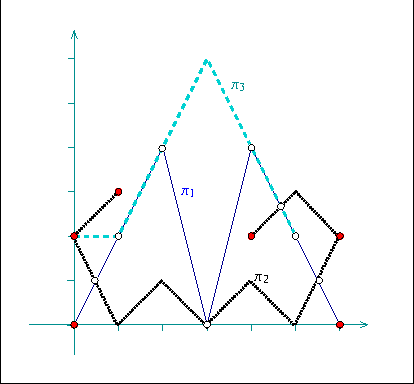
\includegraphics{Arrangement_on_surface_2/fig/ex_12}
  \end{center}
\end{ccTexOnly}
\begin{ccHtmlOnly}
  <p><center>
  <img src="./fig/ex_12.gif" border=0 alt="Example 12">
  </center>
\end{ccHtmlOnly}
\caption{An arrangement of three polylines, as constructed in
\ccc{polylines.cpp}. Disks mark vertices associated with
polyline endpoints, while circles mark vertices that correspond
to intersection points. Note that $\pi_2$ is split into three
$x$-monotone polylines, and that $\pi_1$ and $\pi_3$ have two
overlapping sections.\label{arr_fig:ex_12}}
\end{figure}

The following example program constructs an arrangement of three
polylines, as depicted in Figure~\ref{arr_fig:ex_12}. Note that
most points defining the polylines are not associated with arrangement
vertices. The arrangement vertices are either the extreme points of
each $x$-monotone polyline or the intersection points between two
polylines:

\ccIncludeExampleCode{Arrangement_on_surface_2/polylines.cpp}

%--------------------------------------------------------------
\subsection{A Traits Class for Circular Arcs and Line Segments
  \label{arr_ssec:tr_circ_seg}}
%--------------------------------------------------------------

Circles and circular arcs are the simplest form of non-linear curves.
We handle circles whose centers have rational coordinates and whose
squared radii is also rational. If we denote the circle center by $(x_0,y_0)$
and its radius by $r$, then the equation of the circle --- that is,
$(x - x_0)^2 + (y - y_0)^2 = r^2$ --- has rational coefficients.
The intersection points of two such circles are therefore solutions
of a quadratic equation with rational coefficients, or algebraic numbers
of degree $2$. The same applies for intersection points between such a
rational circle and a line, or a line segment, with rational coefficients
(a line whose equation is $ax + by + c = 0$, where $a$, $b$ and $c$ are
rational). Such numbers can be expressed as $\alpha + \beta\sqrt{\gamma}$,
where $\alpha$, $\beta$ and $\gamma$ are all rational numbers.

Arrangement of circular arcs and of line segment are very useful, as they
occur in many applications. For example, when dilating a polygon by some
radius we obtain a shape whose boundary is comprised of line segments,
which correspond to dilated polygon edges, and circular arcs, which
result from dilated polygon vertices. Using the arrangement of the
boundary curves it is possible, for example, to compute the union of a set
of dilated polygons.

The \ccc{Arr_circle_segment_traits_2<Kernel>} class-template is designed
for efficient handling of arrangements of circular arcs and line segments.
It is a model of the concepts \ccc{ArrangementTraits_2} and
\ccc{ArrangementDirectionalXMonotoneTraits_2}; the later enables
Boolean set operations. Note that it is not a model of
\ccc{ArrangementLandmarkTraits_2} concept, so it is impossible to
use the landmark point-location strategy. The traits class template 
is parameterized by a geometric kernel, and can handle arrangements of
segments of \ccc{Kernel::Circle_2} objects (full circles are also supported)
or of \ccc{Kernel::Line_2} objects---namely circular arcs and line segments.
It is important to observe that the nested \ccc{Point_2} type defined by the
traits class, whose coordinates are typically algebraic numbers of degree 2,
is {\em not} the same as the \ccc{Kernel::Point_2} type, which is capable of
representing a point with rational coordinates. The coordinates of a
point are represented using the nested \ccc{CoordNT} number-type.

\begin{figure}[t]
\begin{ccTexOnly}
  \begin{center}
  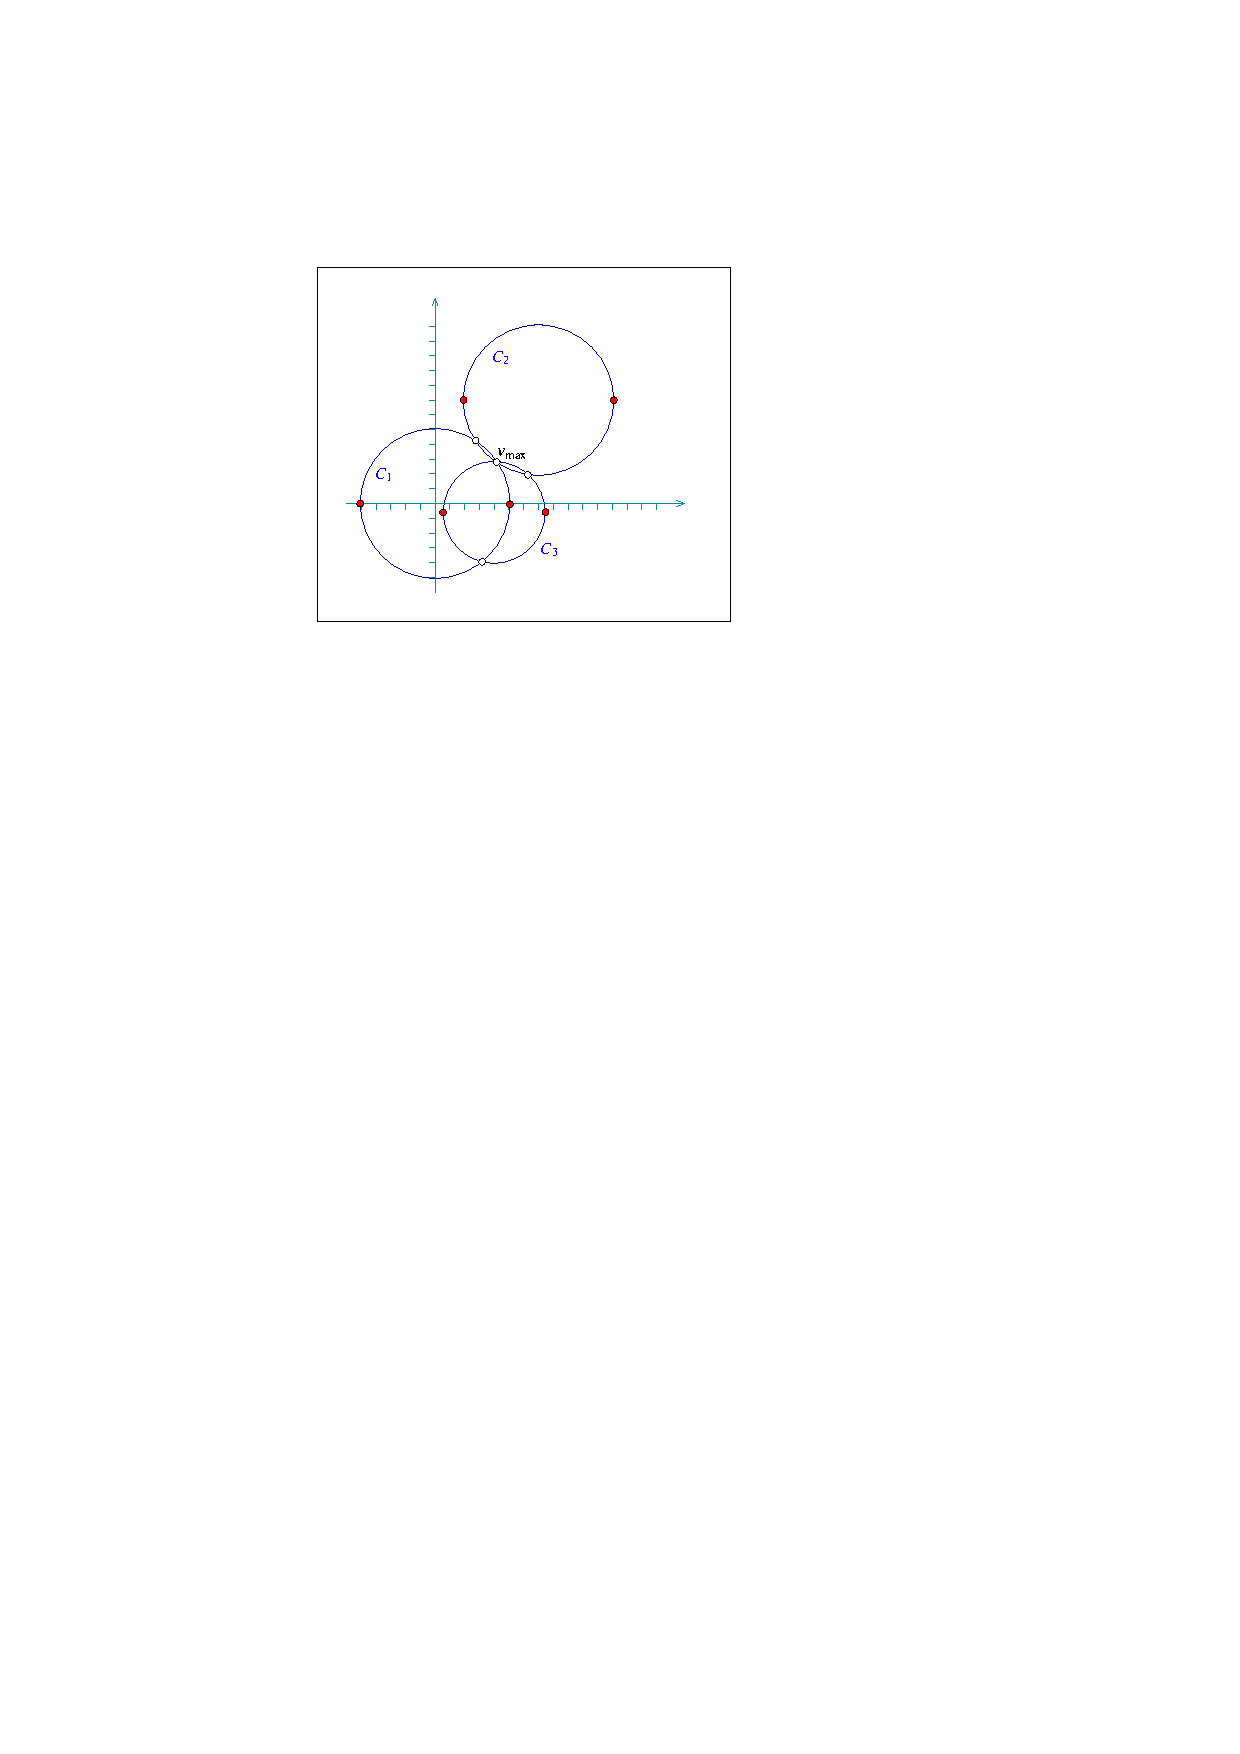
\includegraphics{Arrangement_on_surface_2/fig/ex_13}
  \end{center}
\end{ccTexOnly}
\begin{ccHtmlOnly}
  <p><center>
  <img src="./fig/ex_13.gif" border=0 alt="Example 13">
  </center>
\end{ccHtmlOnly}
\caption{An arrangement of three circles constructed in
\ccc{circles.cpp}. Each circle is split into two $x$-monotone
circular arcs, whose endpoints are drawn as disks. Circles
mark vertices that correspond to intersection points. The vertex
$v_{\rm max}$ is a common intersection point of all three
circles.\label{arr_fig:ex_13}}
\end{figure}

In the following example an arrangement of three full circles is
constructed, as shown in Figure~\ref{arr_fig:ex_13}. Then, the vertex
of maximal degree is searched for. The geometric mapping of this
vertex is the point $(4,3)$, as all three circles intersect at this point
and the associated vertex has six incident edges:

\ccIncludeExampleCode{Arrangement_on_surface_2/circles.cpp}

The \ccc{Curve_2} type nested in \ccc{Arr_circle_segment_traits_2} can be
used to represent circles, circular arcs, or line segments. Curve objects
can therefore be constructed from a \ccc{Kernel::Circle_2} object or from
a \ccc{Kernel::Segment_2} object. A circular arc is typically defined by
a supporting circle and two endpoints, where the endpoints are instances
of the \ccc{Point_2} type, with rational or irrational coordinates. The
orientation of the arc is determined by the orientation of the supporting
circle. Similarly, we also support the construction of lines segments given
their supporting line (of type \ccc{Kernel::Line_2}) and two endpoints, which
may have irrational coordinates (unlike the \ccc{Kernel::Segment_2} type).

Note that the \ccc{Kernel::Circle_2} type represents a circle whose
\emph{squared radius} is rational, where the radius itself may be irrational.
However, if the radius is known to be rational, it is advisable to use it,
for efficiency reasons. It is therefore also possible to construct a circle,
or a circular arc specifying the circle center (a \ccc{Kernel::Point_2}), its
rational radius, and its orientation. Finally, we also support the construction
of a circular arcs that is defined by two endpoints and an arbitrary midpoint
that lies on the arc in between its endpoint. In this case, all three points
are required to have rational coordinates (to be kernel points).

The following example demonstrates the usage of the various construction
methods for circular arcs and line segments. Note the usage of the constructor
of \ccc{CoordNT (alpha, beta, gamma)}, which creates a degree-$2$ algebraic
number whose value is $\alpha + \beta\sqrt{\gamma}$.

\ccIncludeExampleCode{Arrangement_on_surface_2/circular_arcs.cpp}

It is also possible to construct $x$-monotone curve objects, which represent
$x$-monotone circular arcs or line segments, using similar constructors.
Construction from a full circle is obviously not supported. See the Reference
Manual for more details.

The traits class-template
\ccc{Arr_circular_line_arc_traits_2<CircularKernel>} offered by the
arrangement package also handles circular arcs and line segments. It
is an alternative to the \ccc{Arr_circle_segment_traits_2<Kernel>}
class-template. These two class templates, while serve similar
purposes, are based on different concepts, and posses different
characteristics. You are encouraged to experiment with both, compare
their performance, and use the most suitable for your case.

%------------------------------------------------------------------
\subsection{A Traits Class for Conic Arcs\label{arr_ssec:tr_conic}}
%------------------------------------------------------------------

A {\em conic curve} is an algebraic curve of degree 2. Namely, it
is the locus of all points $(x,y)$ satisfying the equation $C:\ r
x^2 + s y^2 + t xy + u x + v y + w = 0$, where the six
coefficients $\langle r, s, t, u, v, w \rangle$ completely
characterize the curve. The sign of the expression $\Delta_{C} = 4
r s - t^2$ determines the type of curve:
\begin{itemize}
\item If $\Delta_{C} > 0$ the curve is an ellipse. A circle is a
special case of an ellipse, where $r = s$ and $t = 0$.
%
\item If $\Delta_{C} = 0$ the curve is a parabola --- an unbounded
conic curve with a single connected branch. When $r = s = t = 0$
we have a line, which can be considered as a degenerate parabola.
%
\item If $\Delta_{C} < 0$ the curve is a hyperbola. That is, it
is comprised of two disconnected unbounded branches.
\end{itemize}

As the arrangement package is suitable for bounded curves, we
consider bounded segments of conic curves, referred to as {\em
conic arcs}. A conic arc $a$ may be either (i) a full ellipse, or
(ii) defined by the tuple $\langle C, p_s, p_t, o \rangle$, where
$C$ is a conic curve and $p_s$ and $p_t$ are two points on $C$
(namely $C(p_s) = C(p_t) = 0$) that define the {\em source} and
{\em target} of the arc, respectively. The arc is formed by
traversing $C$ from the source to the target going in the
orientation specified by $o$, which is typically clockwise or
counterclockwise orientation (but may also be collinear in case of
degenerate conic curves).

We always assume that the conic coefficients $\langle r, s,
t, u, v, w \rangle$ are rational. When dealing with linear curves
(line segments and polylines), similar assumptions guarantee that
all intersection points also have rational coordinates, such that
the arrangement of such curves can be constructed and maintained
using only rational arithmetic. Unfortunately, this does not hold
for conic curves, as the coordinates of intersection points of two
conic curves with rational coefficients are in general algebraic
numbers of degree $4$.\footnote{Namely, they are roots of
polynomials with integer coefficients of degree $4$. However, in
some special cases, for example when handling only circles and
circular arcs, the coordinates of the intersection points are only
of degree $2$, namely they are solutions of quadratic equations.}
In addition, conic arcs may not necessarily be $x$-monotone, and
must be split at points where the tangent to the arc is vertical.
In the general case, such points typically have coordinates that
are algebraic numbers of degree $2$.
It is therefore clear that we have to use different number types
to represent the conic coefficients and the point coordinates.
Note that as arrangement vertices induced by intersection points
and points with vertical tangents are likely to have algebraic
coordinates, we also allow the original endpoints of the input arcs
$p_s$ and $p_t$ to have algebraic coordinates.

The \ccc{Arr_conic_traits_2<RatKernel, AlgKernel, NtTraits>} class
template is designed for efficient handling of arrangements of
bounded conic arcs. The template has three parameters, defined as
follows:
\begin{itemize}
\item The \ccc{RatKernel} class is a geometric kernel, whose field
type is an exact rational type. It is used to define basic
geometric entities (e.g., a line segment or a circle) with rational
coefficients. Typically we use one of the standard \cgal\ kernels,
instantiated with the number type \ccc{NtTraits::Rational} (see
below).
%
\item The \ccc{AlgKernel} class is a geometric kernel whose field
type is an exact algebraic type. It is used to define points with
algebraic coordinates. Typically we use one of the standard
\cgal\ kernels, instantiated with the number type
\ccc{NtTraits::Algebraic} (see below).
%
\item The \ccc{NtTraits} class (the number-type traits class)
encapsulates all the numeric operations needed for performing the
geometric computation carried out by the geometric traits class.
It defines the \ccc{Integer}, \ccc{Rational} and \ccc{Algebraic}
number-types, and supports several operations on these types, such
as conversion between number types, solving quadratic equations
and extracting the real roots of a polynomial with integer
coefficients. It is highly recommended to use the
\ccc{CORE_algebraic_number_traits} class, which is included in the
arrangement package. It relies on the exact number types
implemented in the {\sc Core} library and performs exact
computations on the number types it defines.
\end{itemize}

The \ccc{Arr_conic_traits_2} models the \ccc{ArrangementTraits_2} and
\ccc{ArrangementLandmarkTraits_2} concepts. (It supports
the landmark point-location strategy). Its \ccc{Point_2} type is
derived from \ccc{AlgKernel::Point_2}, while the \ccc{Curve_2}
type represents a bounded, not necessarily $x$-monotone, conic arc.
The \ccc{X_monotone_curve_2} type is derived from \ccc{Curve_2},
but its constructors are to be used only by the traits class.
You should therefore construct only \ccc{Curve_2} objects and
insert them into the arrangement using the \ccc{insert()}
or \ccc{insert()} functions.

Conic arcs can be constructed from full ellipses or by specifying
a supporting curve, two endpoints and an orientation. However,
several constructors of \ccc{Curve_2} are available to allow for some
special cases, such as circular arcs or line segments. The
\ccc{Curve_2} (and the derived \ccc{X_monotone_curve_2}) classes
also support basic access functions such as \ccc{source()},
\ccc{target()} and \ccc{orientation()}.

%~~~~~~~~~~~~~~~~~~~~~~~~~~~~~~~~~~~~~~~~~~~~~~~~~~
\subsubsection{Examples for Arrangements of Conics}
%~~~~~~~~~~~~~~~~~~~~~~~~~~~~~~~~~~~~~~~~~~~~~~~~~~

\begin{figure}[t]
\begin{ccTexOnly}
  \begin{center}
  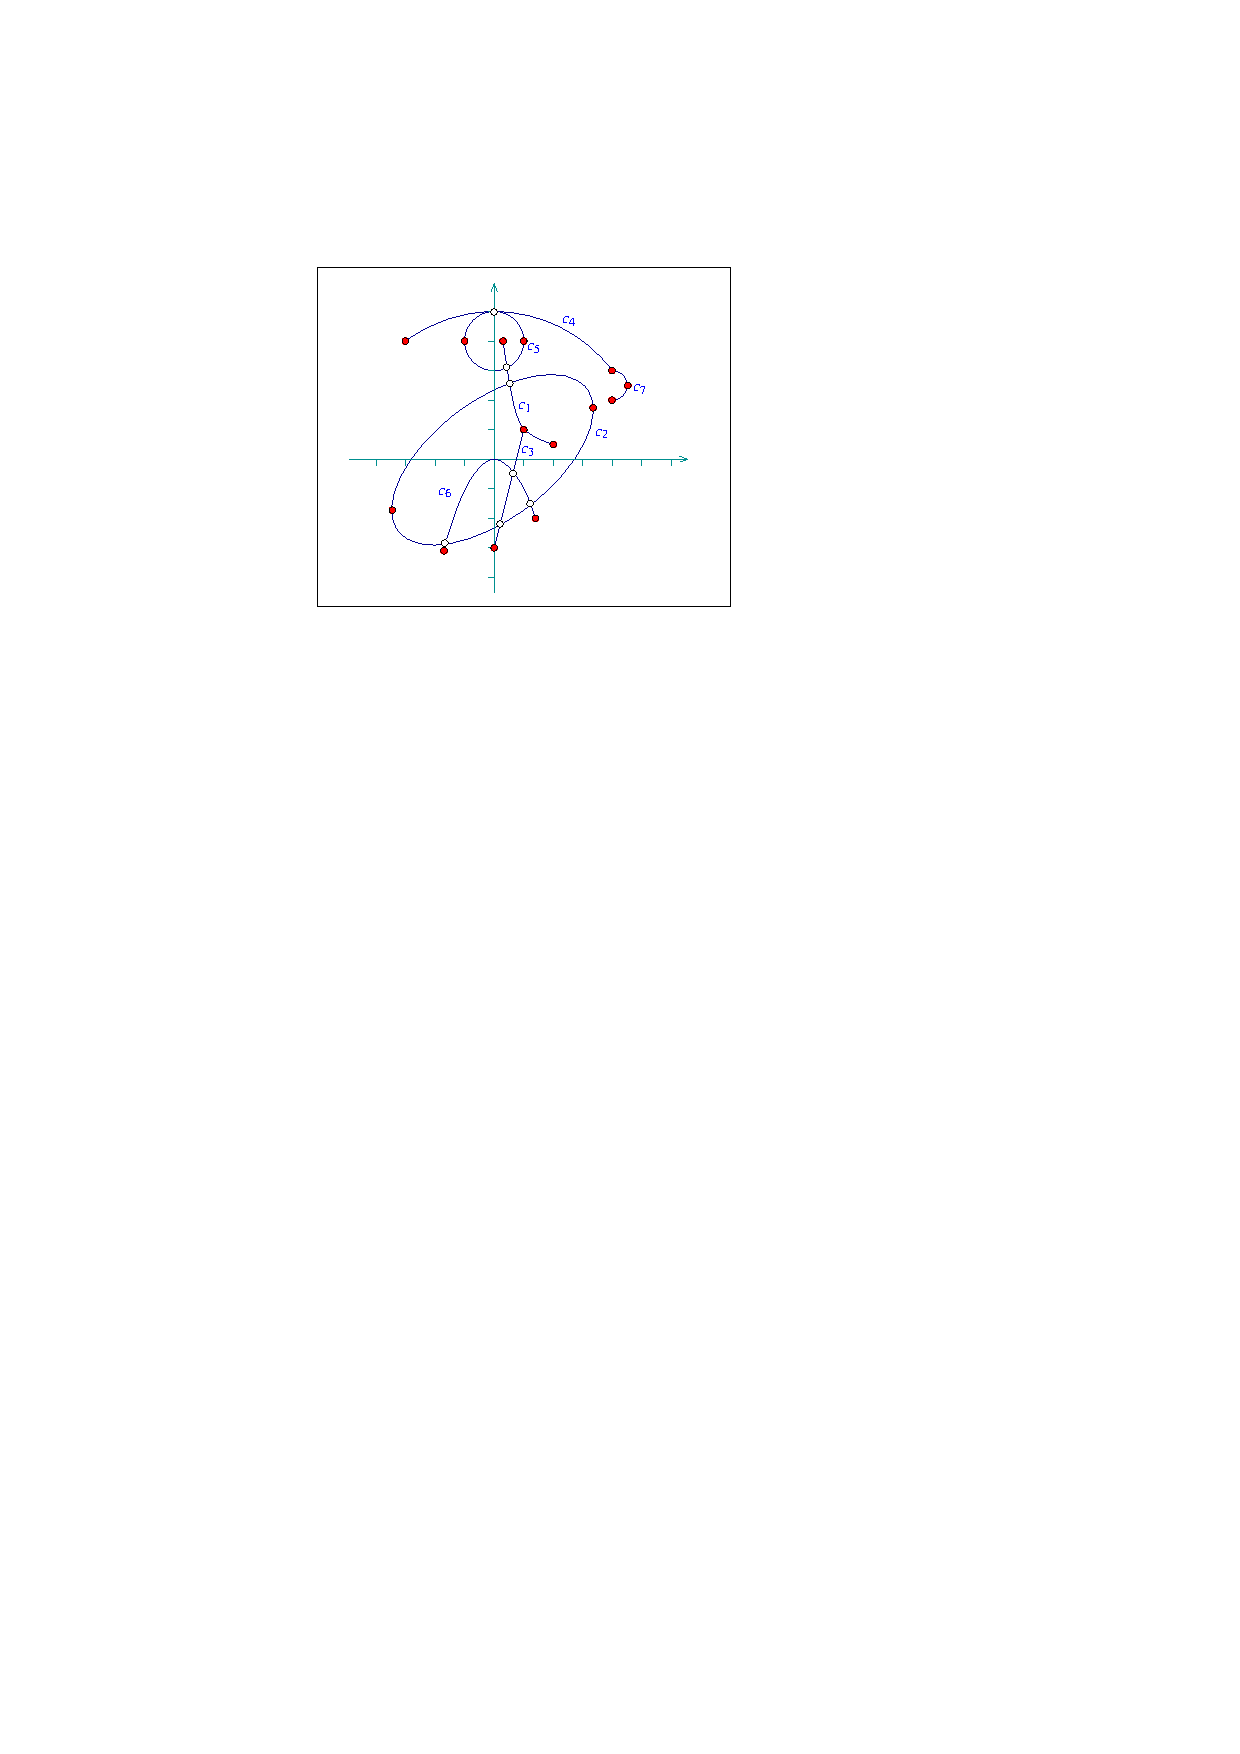
\includegraphics{Arrangement_on_surface_2/fig/ex_14}
  \end{center}
\end{ccTexOnly}
\begin{ccHtmlOnly}
  <p><center>
  <img src="./fig/ex_14.gif" border=0 alt="Example 14">
  </center>
\end{ccHtmlOnly}
\caption{An arrangement of mixed conic arcs, as constructed in
\ccc{conics.cpp}.\label{arr_fig:ex_14}}
\end{figure}

The following example demonstrates the usage of the various
constructors for conic arcs. The resulting arrangement is depicted
in Figure~\ref{arr_fig:ex_14}. Especially noteworthy are the
constructor of a circular arc that accepts three points and the
constructor that allows specifying approximate endpoints, where the
exact endpoints are given explicitly as intersections of
the supporting conic with two other conic curves. Also note that as the
preconditions required by some of these constructors are rather
complicated (see the Reference Manual for the details), a
precondition violation does not cause the program to terminate ---
instead, an {\em invalid} arc is created. We can verify the validity
of an arc by using the \ccc{is_valid()} method. Needless to say, inserting
invalid arcs into an arrangement is not allowed.

\ccIncludeExampleCode{Arrangement_on_surface_2/conics.cpp}

The last example in this section demonstrates how the conic-traits
class can handle intersection points with multiplicity. The
supporting curves of the two arcs, a circle centered at
$(0,\frac{1}{2})$ with radius $\frac{1}{2}$, and the hyperbola $y
= \frac{x^2}{1-x}$,\footnote{This curve can also be written as $C:
x^2 + xy - y = 0$. It is a hyperbola since $\Delta_{C} = -1$.}
intersect at the origin such that the intersection point has
multiplicity $3$ (note that they both have the same horizontal
tangent at $(0,0)$ and the same curvature $1$). In addition, they
have another intersection point at $(\frac{1}{2},\frac{1}{2})$ of
multiplicity $1$:

\ccIncludeExampleCode{Arrangement_on_surface_2/conic_multiplicities.cpp}

%---------------------------------------------------------
\subsection{A Traits Class for Arcs of Rational Functions\label{arr_ssec:tr_ratfunc}}
%---------------------------------------------------------

The traits class
\ccc{Arr_rational_function_traits_2<AlgebraicKernel_d_1>} handles
bounded and unbounded arcs of rational functions, referred to as
\emph{rational arcs} (in particular, such an arc may correspond to the
entire graph of a rational function), and enables the construction and
maintenance of arrangements of such arcs. Rational functions, and
polynomial functions in particular, are not only interesting in their
own right, they are also very useful for approximating or
interpolating more complicated curves; see,
e.g.,~\cite[Chapter~3]{cgal:ptvf-nrcpp-02}.

\ccc{Arr_rational_function_traits_2<AlgebraicKernel_d_1>} is a model
of the concepts \ccc{ArrangementTraits_2},
\ccc{ArrangementOpenBoundaryTraits_2}, and
\ccc{ArrangementDirectionalXMonotoneTraits_2}; the later enables
Boolean set operations. Note that it is not a model of
\ccc{ArrangementLandmarkTraits_2} concept, so it is impossible to use
the landmark point-location strategy with this traits class.
%\footnote{This requires a relaxation of \ccc{ArrangementLandmarkTraits_2}, 
%which will be submitted separately.}

A rational function $y = \frac{P(x)}{Q(x)}$ is defined by two
polynomials $P$ and $Q$ of arbitrary degrees.  If $Q(x) = 1$ then
the function is a simple polynomial function. Usually the domain is
$\R$ but the function may also be restricted to a bounded interval
$[x_{\rm min}, x_{\rm max}]$ or defined over a ray
$(-\infty, x_{\rm max}]$ or $[x_{\rm min}, \infty)$. Rational
functions are represented by the nested type \ccc{Curve_2}.
A rational arc is always $x$-monotone in the mathematical
sense. However, it is not necessarily continuous, as it may have
singularities. An arc that has singularities must 
be split into continuous portions before being inserted into the
arrangement. Arbitrary rational functions are represented by the 
nested type \ccc{Curve_2} and continuous portions of rational
functions are represented by the nested type
\ccc{X_monotone_curve_2}. Constructors for both types are provided by
the traits. A \ccc{Curve_2} may be split up into several
\ccc{X_monotone_curve_2} using \ccc{Make_x_monotone_2}.

Using the \ccc{Arr_rational_function_traits_2<AlgebraicKernel_d_1>}
class template it is possible to construct and maintain arrangement
of rational arcs. The template parameter of the traits must be a model
of the concept \ccc{AlgebraicKernel_d_1}. A rational function is
represented as the quotient of two polynomials $P$ and $Q$ of type
\ccc{AlgebraicKernel_d_1::Polynomial_1} and an $x$-interval over which
the polynomials are defined. The type of the polynomial coefficients,
namely \ccc{AlgebraicKernel_d_1::Coefficient}, cannot be algebraic.
Moreover, it is recommended that this type is not made rational either,
since using rational, as opposed to integral, coefficients does not
extend the range of the rational arcs and is typically less efficient.
The type of the interval bounds, namely
\ccc{AlgebraicKernel_d_1::Bound}, however, can be algebraic. A point is
represented by a rational function and its $x$-coordinate, which is of
type \ccc{AlgebraicKernel_d_1::Algebraic_real_1}. Note that an explicit
representation of the $y$-coordinate is only computed upon request, as
it can be a rather costly operation.

The constructed rational functions are cached by the traits class. The
cache is local to each traits class object. It is therefore necessary
to construct curves using only the constructor objects provided by
member functions of the traits class.
%This is also the reason why IO is not handled via the usual stream operators. 
Moreover, a curve must only be used by the traits class object that
was used to construct it. The cache is automatically cleaned up from
time to time. The amortized clean up costs are constant. In addition,
there is also a separate member function that cleans up the cache on
demand.

The curve constructors have an additional advantage. They conveniently
enable the provision of two polynomials that define a rational arc
using rational coefficients. For example, let $P$ and $Q$ denote two
polynomials with integral coefficients that define a rational arc at
interest, and let $P'$ and $Q'$ denote two polynomials with rational
coefficients that define the same rational arc; that is, the quotients
$P/Q$ and $P'/Q'$ are identical. You can construct the rational arc
providing the coefficients of $P'$ and $Q'$ to the constructor. In this
case the constructor normalizes the coefficients and stores the desired
polynomials $P$ and $Q$.

\begin{figure}[ht]
\begin{ccTexOnly} 
  \begin{center}
  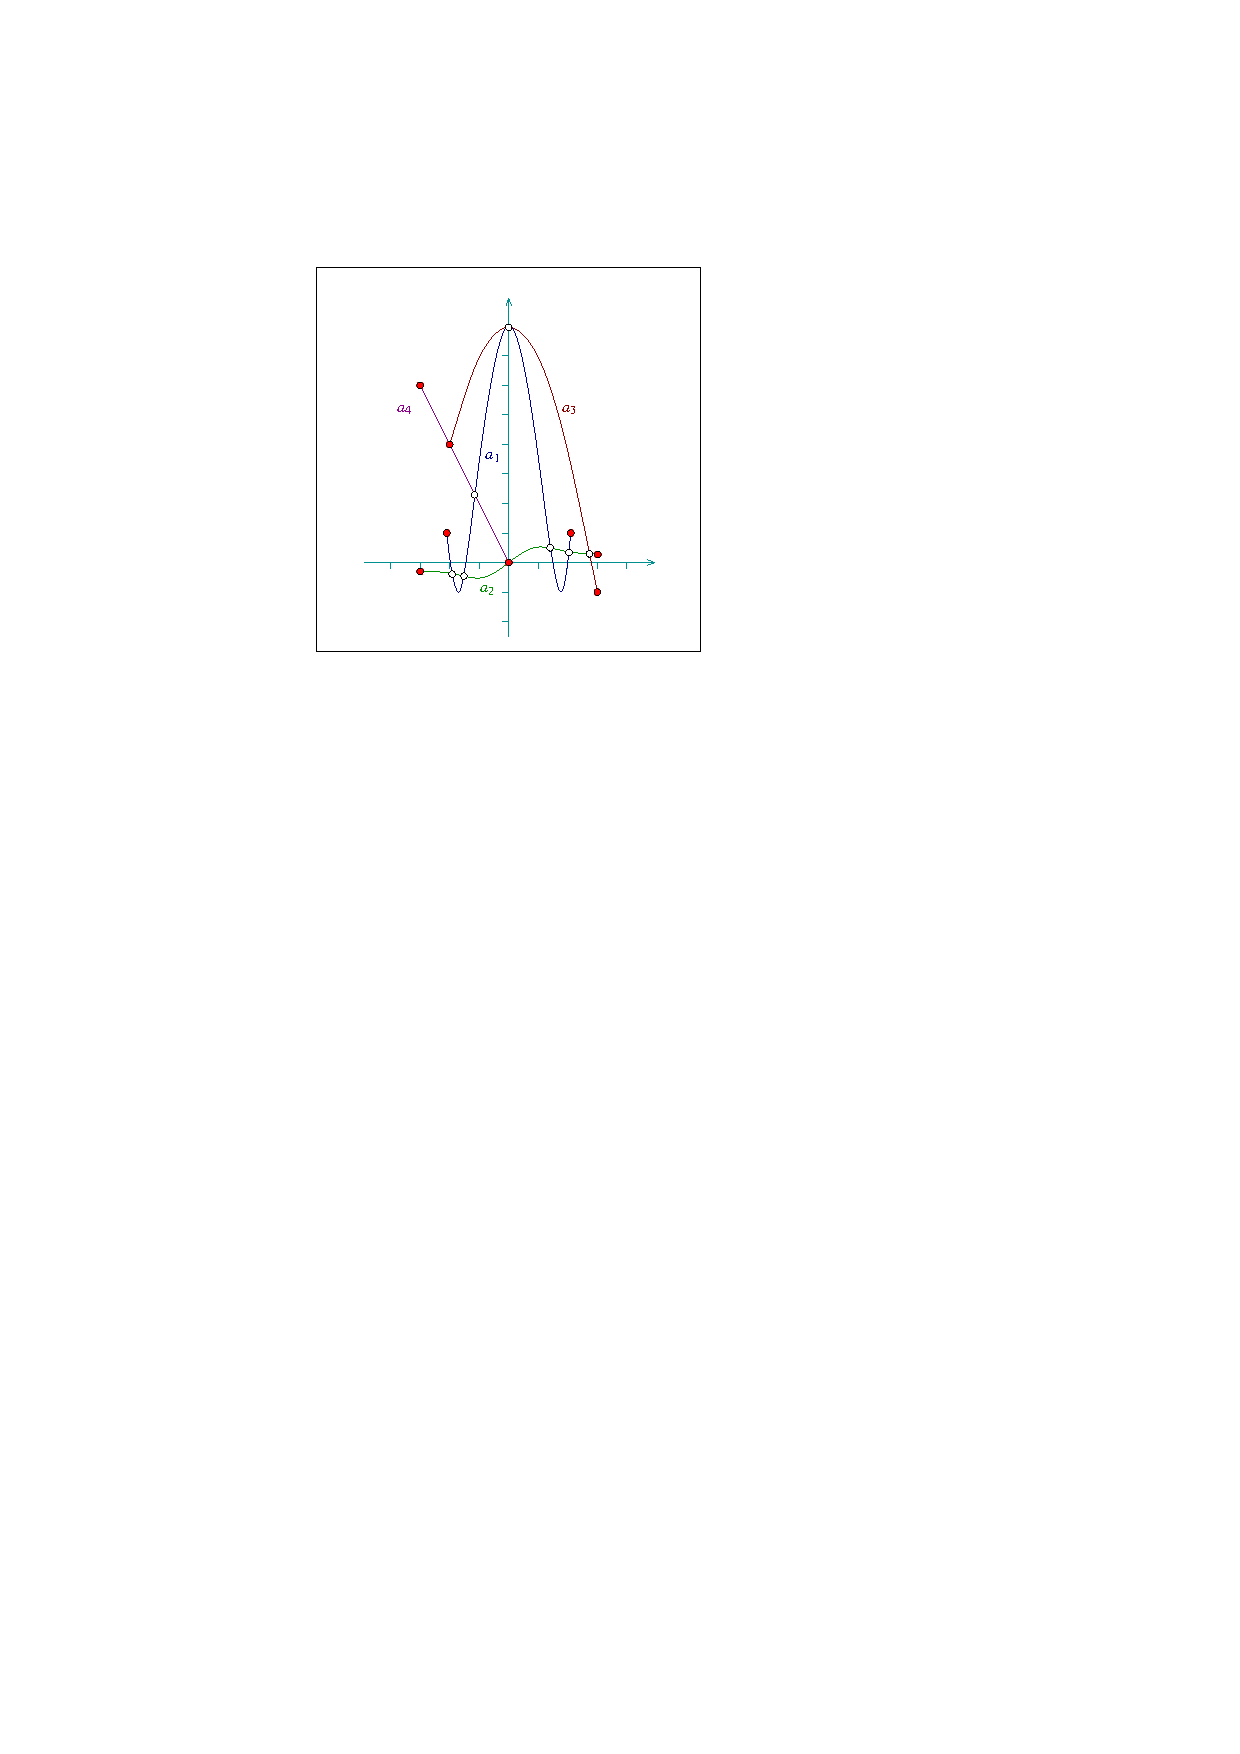
\includegraphics{Arrangement_on_surface_2/fig/ex_16}
  \end{center}
\end{ccTexOnly}
\begin{ccHtmlOnly}
  <p><center>
  <img src="./fig/ex_16.gif" border=0 alt="Example 16">
  </center>
\end{ccHtmlOnly}
\caption{An arrangement of four arcs of rational functions, as
constructed in \ccc{rational_functions.cpp}.\label{arr_fig:ex_16}}
\end{figure}

The following example demonstrates the construction of an
arrangement of rational arcs depicted in
Figure~\ref{arr_fig:ex_16}. Note the usage of the two
constructors, for polynomial arcs and for rational arcs:

\pagebreak[3]

\ccIncludeExampleCode{Arrangement_on_surface_2/rational_functions.cpp}

\begin{figure}[ht]
\begin{ccTexOnly}
  \begin{center}
  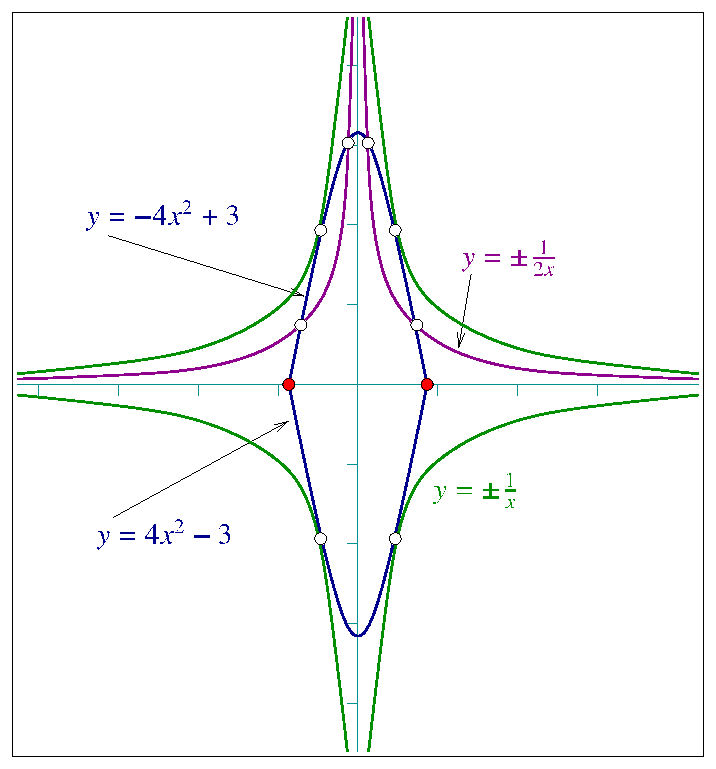
\includegraphics{Arrangement_on_surface_2/fig/ex_unb_rat}
  \end{center}
\end{ccTexOnly}
\begin{ccHtmlOnly}
  <p><center>
  <img src="./fig/ex_unb_rat.gif" border=0 alt="">
  </center>
\end{ccHtmlOnly}
\caption{An arrangement of six arcs of rational functions, as
constructed in
\ccc{unbounded_rational_functions.cpp}.\label{arr_fig:ex_unb_rat}}
\end{figure}

The following example demonstrates the construction of an
arrangement of six rational arcs---four unbounded arcs and two
bounded ones---as depicted in Figure~\ref{arr_fig:ex_unb_rat}. Note
the usage of the constructors of an entire rational function and of
an infinite ``ray'' of such a function. Also observe that the hyperbolas
$y = \pm\frac{1}{x}$ and $y = \pm\frac{1}{2x}$ never intersect, although
they have common vertical and horizontal asymptotes, so very ``thin''
unbounded faces are created between them:

\ccIncludeExampleCode{Arrangement_on_surface_2/unbounded_rational_functions.cpp}

%----------------------------------------------------------------------------
\subsection{A Traits Class for Planar B\'ezier Curves\label{arr_ssec:tr_bez}}
%----------------------------------------------------------------------------

A planar {\em B\'ezier curve} $B$ is a parametric curve defined by a sequence
of {\em control points} $p_0, \ldots, p_n$ as follows:
\begin{eqnarray*}
B(t) = \left(X(t), Y(t)\right)
  = \ccSum{k=0}{n}{p_k \cdot \frac{n!}{k! (n-k)!} \cdot
                   t^k (1-t)^{n-k}}\ .
\end{eqnarray*}
where $t \in [0, 1]$. The degree of the curve is therefore $n$ ---
namely, $X(t)$ and $Y(t)$ are polynomials of degree $n$. B\'ezier curves
have numerous applications in computer graphics and solid modelling. They
are used, for example, in free-form sketches and for defining the true-type
fonts.

Using the \ccc{Arr_Bezier_curve_traits_2<RatKernel, AlgKernel, NtTraits>}
class template it is possible to construct and maintain arrangements of
B\'ezier curves that are given by rational control points (a sequence
of objects of the \ccc{RatKernel::Point_2} type). We can handle curves
of arbitrary degree (in general, a sequence of $n+1$ control points define a 
B\'ezier curve of degree $n$). The template parameters are the same ones
used by the \ccc{Arr_conic_traits_2} class template, and here it is also
recommended to use the \ccc{CORE_algebraic_number_traits} class, with
Cartesian kernels instantiated with the \ccc{Rational} and \ccc{Algebraic}
number-types defined by this class.

As mentioned above, we assume that the coordinates of all control
points that define a B\'ezier curve are rational numbers, so both $X(t)$
and $Y(t)$ are polynomials with rational coefficients. The intersection
points between curves are however algebraic numbers, and their exact
computation is time-consuming. The traits class therefore contains a layer
of geometric filtering that performs all computation in an approximate
manner whenever possible. Thus, it resorts to exact computations only when
the approximate computation fails to produce an unambiguous result.
Note that most arrangement vertices are therefore associated with approximated
points. You cannot access the coordinates of such points and obtain them as
algebraic numbers, and only access to the approximate coordinates in possible.
See the Reference Manual for the exact interface of the \ccc{Point_2},
\ccc{Curve_2} and \ccc{X_monotone_curve_2} defined by the traits class.

The \ccc{Arr_Bezier_curve_traits_2} is a model of the
\ccc{ArrangementTraits_2} concept (but not of the
\ccc{ArrangementLandmarkTraits_2} concept, so it is impossible
to use the landmark point-location strategy for arrangements of
rational arcs).

\begin{figure}[t]
\begin{ccTexOnly}
  \begin{center}
  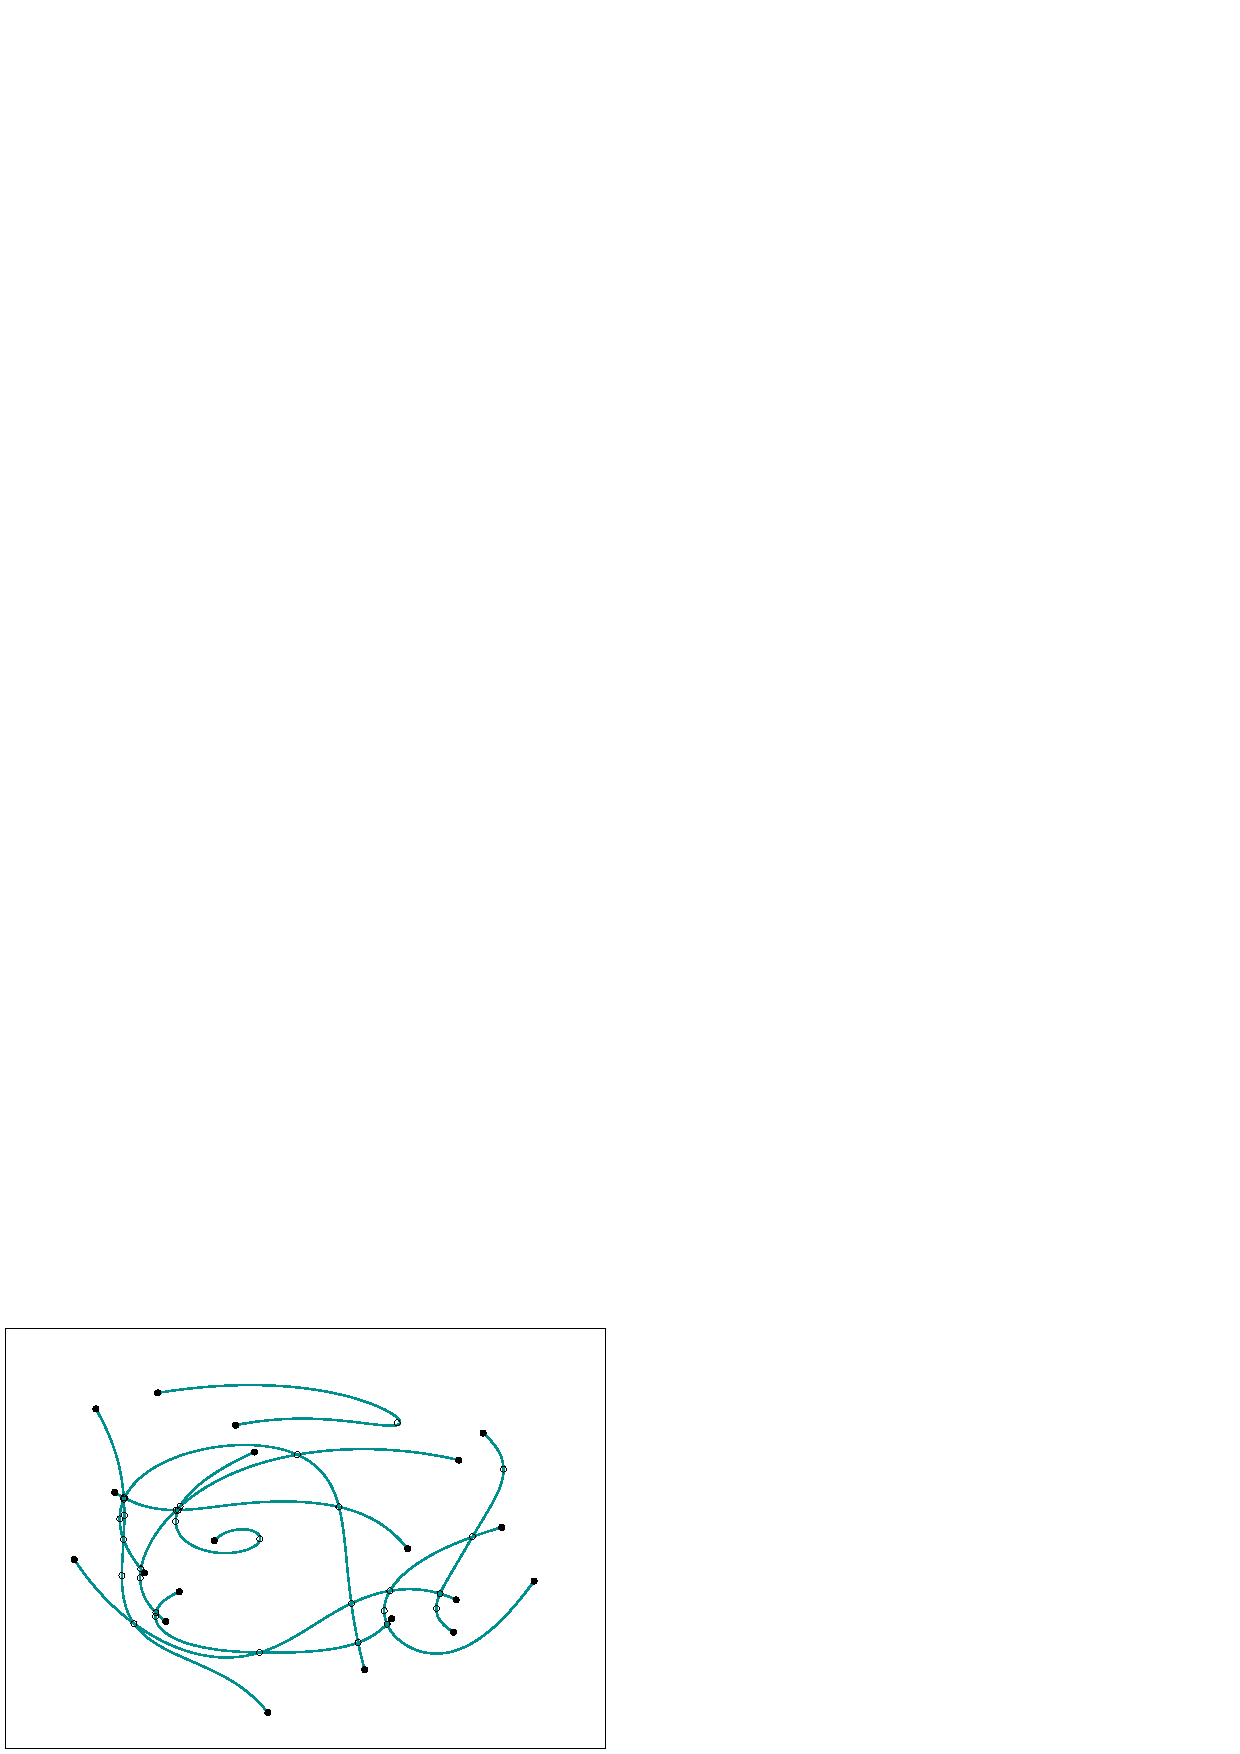
\includegraphics{Arrangement_on_surface_2/fig/Bezier_arr}
  \end{center}
\end{ccTexOnly}
\begin{ccHtmlOnly}
  <p><center>
  <img src="./fig/Bezier_arr.gif" border=0 alt="An arrangement of Bezier curves">
  </center>
\end{ccHtmlOnly}
\caption{An arrangement of ten B\'ezier curves of degree $5$, as
constructed in \ccc{Bezier_curves.cpp}.\label{arr_fig:ex_bez}}
\end{figure}

The following example reads a set of B\'ezier curves from an input
file, where each file is specified by an integer stating its number
of control points, followed by the sequence of control points, given
in integer or rational coordinates. By default, the program uses
the \ccc{Bezier.dat} file, which contains ten curves of degree $5$
each; their resulting arrangement is depicted in
Figure~\ref{arr_fig:ex_bez}.

\ccIncludeExampleCode{Arrangement_on_surface_2/Bezier_curves.cpp}

%-------------------------------------------------------------------------
\subsection{A Traits Class for Planar Algebraic Curves of Arbitrary Degree
  \label{arr_ssec:tr_alg}}
%-------------------------------------------------------------------------

An algebraic curve $C$ in the plane is defined as the (real) zero locus
of a polynomial $f(x,y)$ in two variables. The curve is uniquely defined
by $f$ (although several polynomials might define the same curve). 
We call $f$ a \emph{defining polynomial} of $C$.

% When talking about algebraic curves, we use the term ``segment'' for a
% closed continuous subset of an algebraic curve
% such that each interior point can be parameterized uniquely, as a function in
% $x$ or $y$. In other words, there is no self-intersection in the interior
% of a segment. A weakly $x$-monotone segment is therefore a segment that is
% either vertical, or permits a unique parameterization
We consider arrangements induced by algebraic curves
or by (weakly) $x$-monotone segments for algebraic curves
(Such a segment is not necessarily the maximal possible 
(weakly) x-monotone segment; see below.)
When talking about algebraic curves, 
we use the term ``segment'' for a continuous, possibly non-linear subset 
of an algebraic curve~-- see the definition below.
There are no restrictions on the algebraic curve, that means, 
we support unbounded curves, vertical curves or segments, and isolated points.

The \ccc{Arr_algebraic_segment_traits_2<Coefficient>} class template 
is a model of the \ccc{ArrangementTraits_2} concept (but not of the
\ccc{ArrangementLandmarkTraits_2} concept, so it is impossible
to use the landmark point-location strategy for arrangements of
algebraic curves).
The template argument \ccc{Coefficient} determines 
the type of the scalar coefficients of the polynomial. 
Currently supported types are \ccc{leda_integer}, \ccc{CORE::BigInt}, 
and any instance of \ccc{CGAL::Sqrt_extension<A,B>} 
instantiated with one of the integral types above.

The traits class defines a type \ccc{Curve_2} for algebraic curves.
Such a type can be constructed by the \ccc{Construct_curve_2} functor,
which accepts an instance of \ccc{Polynomial_2} as an argument.
This polynomial type is also available by the traits class 
and constitutes a valid model
of the concept \ccc{Polynomial_d} with two variables (see~??).
%The \ccc{Construct_curve_2} functor performs a topological-geometric analysis
%of the defined curve, and caches the result internally.

\begin{figure}[t]
\begin{ccTexOnly}
  \begin{center}
  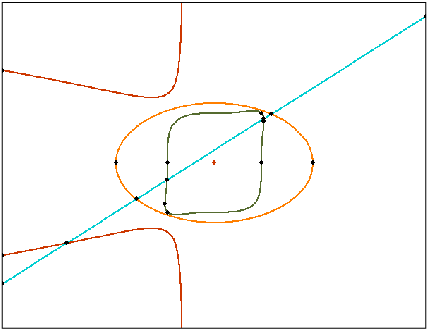
\includegraphics[width=8cm]{Arrangement_on_surface_2/fig/algebraic_curves}
  \end{center}
\end{ccTexOnly}
\begin{ccHtmlOnly}
  <p><center>
  <img src="./fig/algebraic_curves.gif" border=0 alt="An arrangement of algebraic curves">
  </center>
\end{ccHtmlOnly}
\caption{An arrangement of algebraic curves of degrees $1$, $2$, $3$, and $6$,
as constructed in \ccc{algebraic_curves.cpp}.\label{arr_fig:ex_alg_curves}}
\end{figure}

The following examples computes the arrangement induced by the four curves
in Figure~\ref{arr_fig:ex_alg_curves}

\ccIncludeExampleCode{Arrangement_on_surface_2/algebraic_curves.cpp}

We first give a precise definition of segments of algebraic curves.
A point $p$ on a curve $C_f\subset\mathbb{R}^2$ 
(with $f$ its defining equation) is called
\emph{semi-regular}, if locally around $p$, $C_f$ can be written as
a function graph of some continuous function in $x$ or in $y$
(we also say that $p$ is parameterizable in $x$ or $y$, respectively).
The only two cases of non-semi-regular points are isolated points, and
self-intersections. 
A \emph{segment} of a curve is a closed and continuous point set 
such that each interior point is semi-regular.
It follows that a weakly $x$-monotone segment is either a completely vertical
segment, or a segment whose interior points are all parameterizable in $x$.

The traits class allows to construct weakly $x$-monotone segments of a curve
using the \ccc{Construct_x_monotone_segment_2} functor.
The \ccc{X_monotone_curve_2} type of the traits class represents
weakly $x$-monotone segments of a curve; however,
segments may need to be further subdivided into several (sub-)segments,
for technical reasons. Therefore, \ccc{Construct_x_monotone_segment_2}
constructs a sequence of \ccc{X_monotone_curve_2} objects, whose union
represents the weakly $x$-monotone segment that was queried.
We call a segment \emph{terminal} if it can be represented
by the type \ccc{X_monotone_curve_2}.

\begin{ccAdvanced}
The subdivision of segments is due to the internal representation of 
$x$-monotone segments, which is based on a vertical decomposition.
We assume the defining polynomial $f$ of the curve $C$
to be \emph{square-free}, that means, it contains no divisor $g^2$ of total
degree greater than zero. We define a \emph{(complex) critical point}
$p\in\mathbb{C}^2$ by
%
$$f(p)=0=\frac{\partial f}{\partial y}(p).$$
%
An $x$-coordinate $\alpha\in\mathbb{R}$ is \emph{critical}
if either some critical point has $x$-coordinate $\alpha$,
or if the leading coefficient of $f$, considered as a polynomial in $y$,
vanishes. In particular, vertical lines of and isolated point of $C$
can only take place at critical $x$-coordinates.
Between two consecutive critical $x$-coordinates, the curve decomposes
into a finite number of $x$-monotone segments (the same is true on the left
of the leftmost, and on the right of the rightmost critical $x$-coordinate).
The type \ccc{X_monotone_curve_2} is only able to represent such segments
(and sub-segments of them). See Figure~\ref{arr_fig:cylindrical_decomposition} 
for an example of a decomposition into terminal segments. Formally, 
a terminal segment is a weakly $x$-monotone segment that is either vertical, or
its $x$-range contains no critical point in its interior.

\end{ccAdvanced}

\begin{figure}[t]
\begin{ccTexOnly}
 \begin{center}
 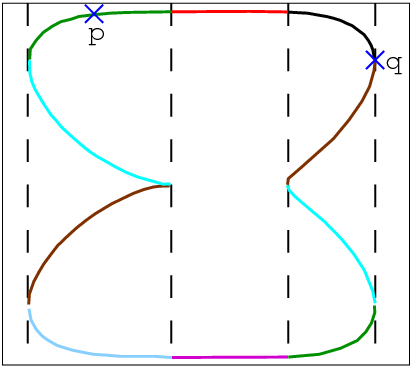
\includegraphics[width=8cm]{Arrangement_on_surface_2/fig/cylindrical_decomposition}
 \end{center}
\end{ccTexOnly}
\begin{ccHtmlOnly}
 <p><center>
 <img src="./fig/cylindrical_decomposition.gif" border=0 alt="The algebraic curves">
 </center>
\end{ccHtmlOnly}
\caption{The critical $x$-coordinates of an algebraic curve (dashed lines),
         and its decomposition into terminal segments (in different colors).
         The segment from $p$ to $q$ consists of the union of 
         three terminal segments.
         \label{arr_fig:cylindrical_decomposition}}
\end{figure}

Coordinates of points are represented by the type \ccc{Algebraic_real_1},
which is defined in the traits class. 
This type is taken from a model of the \ccc{AlgebraicKernel_1} concept,
which is also available by the type \ccc{Algebraic_kernel_1}.
One can use this model to create algebraic numbers as roots of univariate
polynomials, and process them, for instance, 
compare them, or approximate them to any precision. See the documentation
of \ccc{AlgebraicKernel_1} for more information.
One can construct an object of type \ccc{Point_2} by a triple
($x_0$,cv,i), which means that the $i$-th point (counted from below)
in the fiber of cv at the $x$-coordinate $x_0$ is constructed.
This is also how points are presented internally. 
In the example displayed in Figure~\ref{arr_fig:cylindrical_decomposition},
if $x_1$ denotes the $x$-coordinate of $p$, and $cv$ represents the algebraic
curve, then $p$ could be represented by $(x_1,cv,3)$. If $x_2$
is the $x$-coordinate of $q$, 
then $(x_2,cv,1)$ is a valid representation of $q$.
Although the $y$-coordinate of an object of type \ccc{Point_2} can be queried,
we recommend to be careful with that option, since computing an explicit
representation of the $y$-coordinate as an \ccc{Algebraic_real_1} object
can become rather expensive.

\begin{figure}[t]
\begin{ccTexOnly}
 \begin{center}
 
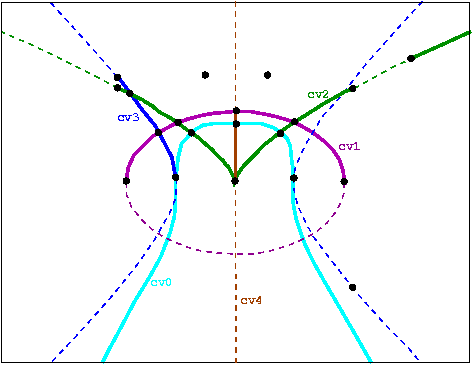
\includegraphics[width=8cm]{Arrangement_on_surface_2/fig/algebraic_segments}
 \end{center}
\end{ccTexOnly}
\begin{ccHtmlOnly}
 <p><center>
 <img src="./fig/algebraic_segments.gif" border=0 alt="An arrangement of algebraic segments">
 </center>
\end{ccHtmlOnly}
\caption{An arrangement of algebraic segments (solid lines),
as constructed in \ccc{algebraic_segments.cpp}. The supporting curves
are drawn in dashed lines.\label{arr_fig:ex_alg_segments}}
\end{figure}

The following code exemplifies various methods to construct
algebraic segments. The computed arrangement is displayed in
Figure~\ref{arr_fig:ex_alg_segments}.

\ccIncludeExampleCode{Arrangement_on_surface_2/algebraic_segments.cpp} 

%-----------------------------------------------------------
\subsection{Traits-Class Decorators\label{arr_ssec:meta_tr}}
%-----------------------------------------------------------

Geometric traits-class decorators allow you to attach auxiliary
data to curves and to points. The data is automatically manipulated 
by the decorators and distributed to the constructed geometric entities. 
Note that additional information can alternatively be maintained by extending 
the vertex, halfedge, or face types provided by the \dcel\ class used 
by the arrangement; see the details in Section~\ref{arr_sec:ex_dcel}.

The arrangement package includes a generic traits-class decorator
template named 
\ccc{Arr_curve_data_traits_2<BaseTraits, XMonotoneCurveData, Merge, CurveData, Convert>}.
This decorator is used to attach a data field to curves and to
$x$-monotone curves. It is parameterized by a base-traits class, which is
one of the geometric traits classes described in the previous subsections, or
a user-defined traits class. The curve-data decorator derives itself from the
base-traits class, and in particular inherits its \ccc{Point_2} type.
In addition:
\begin{itemize}
\item \ccc{Curve_2} is derived from the basic \ccc{BaseTraits::Curve_2}
class, extending it by an extra field of type \ccc{CurveData}.
%
\item \ccc{X_monotone_curve_2} is derived from the basic
\ccc{BaseTraits::X_monotone_curve_2} class, extending it by an extra field of
type \ccc{XMonotoneCurveData}.
\end{itemize}
Note that the \ccc{Curve_2} and \ccc{X_monotone_curve_2} are not
the same, even if the \ccc{BaseTraits::Curve_2} and
\ccc{BaseTraits::X_monotone_curve_2} are (as in the case of the 
segment-traits class for example). The extended curve types support the
additional methods \ccc{data()} and \ccc{set_data()} for
accessing and modifying the data field.

You can create an extended curve (or an extended $x$-monotone curve)
from a basic curve and a curve-data object. When curves are
inserted into an arrangement, they may be split, and the
decorator handles their data fields automatically:
\begin{itemize}
\item When a curve is subdivided into $x$-monotone subcurves, its
data field of type \ccc{CurveData} is converted to an \ccc{XMonotoneCurveData}
object $d$ using the \ccc{Convert} functor. The object $d$ is automatically
associated with each of the resulting $x$-monotone subcurves.

Note that by default, the \ccc{CurveData} type is identical to the
\ccc{XMonotoneCurveData} type (and the conversion functor \ccc{Convert}
is trivially defined). Thus, the data field associated with the original
curve is just duplicated and stored with the $x$-monotone subcurves.
%
\item When an $x$-monotone curve is split into two, the decorator
class automatically copies its data field to both resulting subcurves.
%
\item When intersecting two $x$-monotone curves $c_1$ and $c_2$, the
result may include overlapping sections, represented as
$x$-monotone curves. In this case the data fields of $c_1$ and $c_2$
are merged into a single \ccc{XMonotoneCurveData} object,
using the \ccc{Merge} functor, which is supplied as a
parameter to the traits class-template. The resulting object is
assigned to the data field of the overlapping subcurves.
%
\item Merging two $x$-monotone curves is allowed only when (i)~the two
curves are geometrically mergeable --- that is, the base-traits class
allows to merge them --- and (ii)~the two curves store the same data field.
\end{itemize}

The \ccc{Arr_consolidated_curve_data_traits_2<BaseTraits, Data>} decorator
specializes the generic curve-data decorator. It extends the basic
\ccc{BaseTraits::Curve_2} by a single \ccc{Data} field, and the basic
\ccc{BaseTraits::X_monotone_curve_2} with a {\em set} of (distinct) data 
objects. The \ccc{Data} type is required to support the equality operator, 
used to ensure that each set contains only distinct data objects with no 
duplicates.
When a curve with a data field $d$ is subdivided into $x$-monotone subcurves,
each subcurve is associated with a set $S = \{ d \}$. In case of an overlap
between two $x$-monotone curves $c_1$ and $c_2$ with associated data sets
$S_1$ and $S_2$, respectively, the overlapping subcurve is associated with
the consolidated set $S_1 \cup S_2$.

%~~~~~~~~~~~~~~~~~~~~~~~
\subsubsection{Examples}
%~~~~~~~~~~~~~~~~~~~~~~~

\begin{figure}[t]
\begin{ccTexOnly}
  \begin{center}
  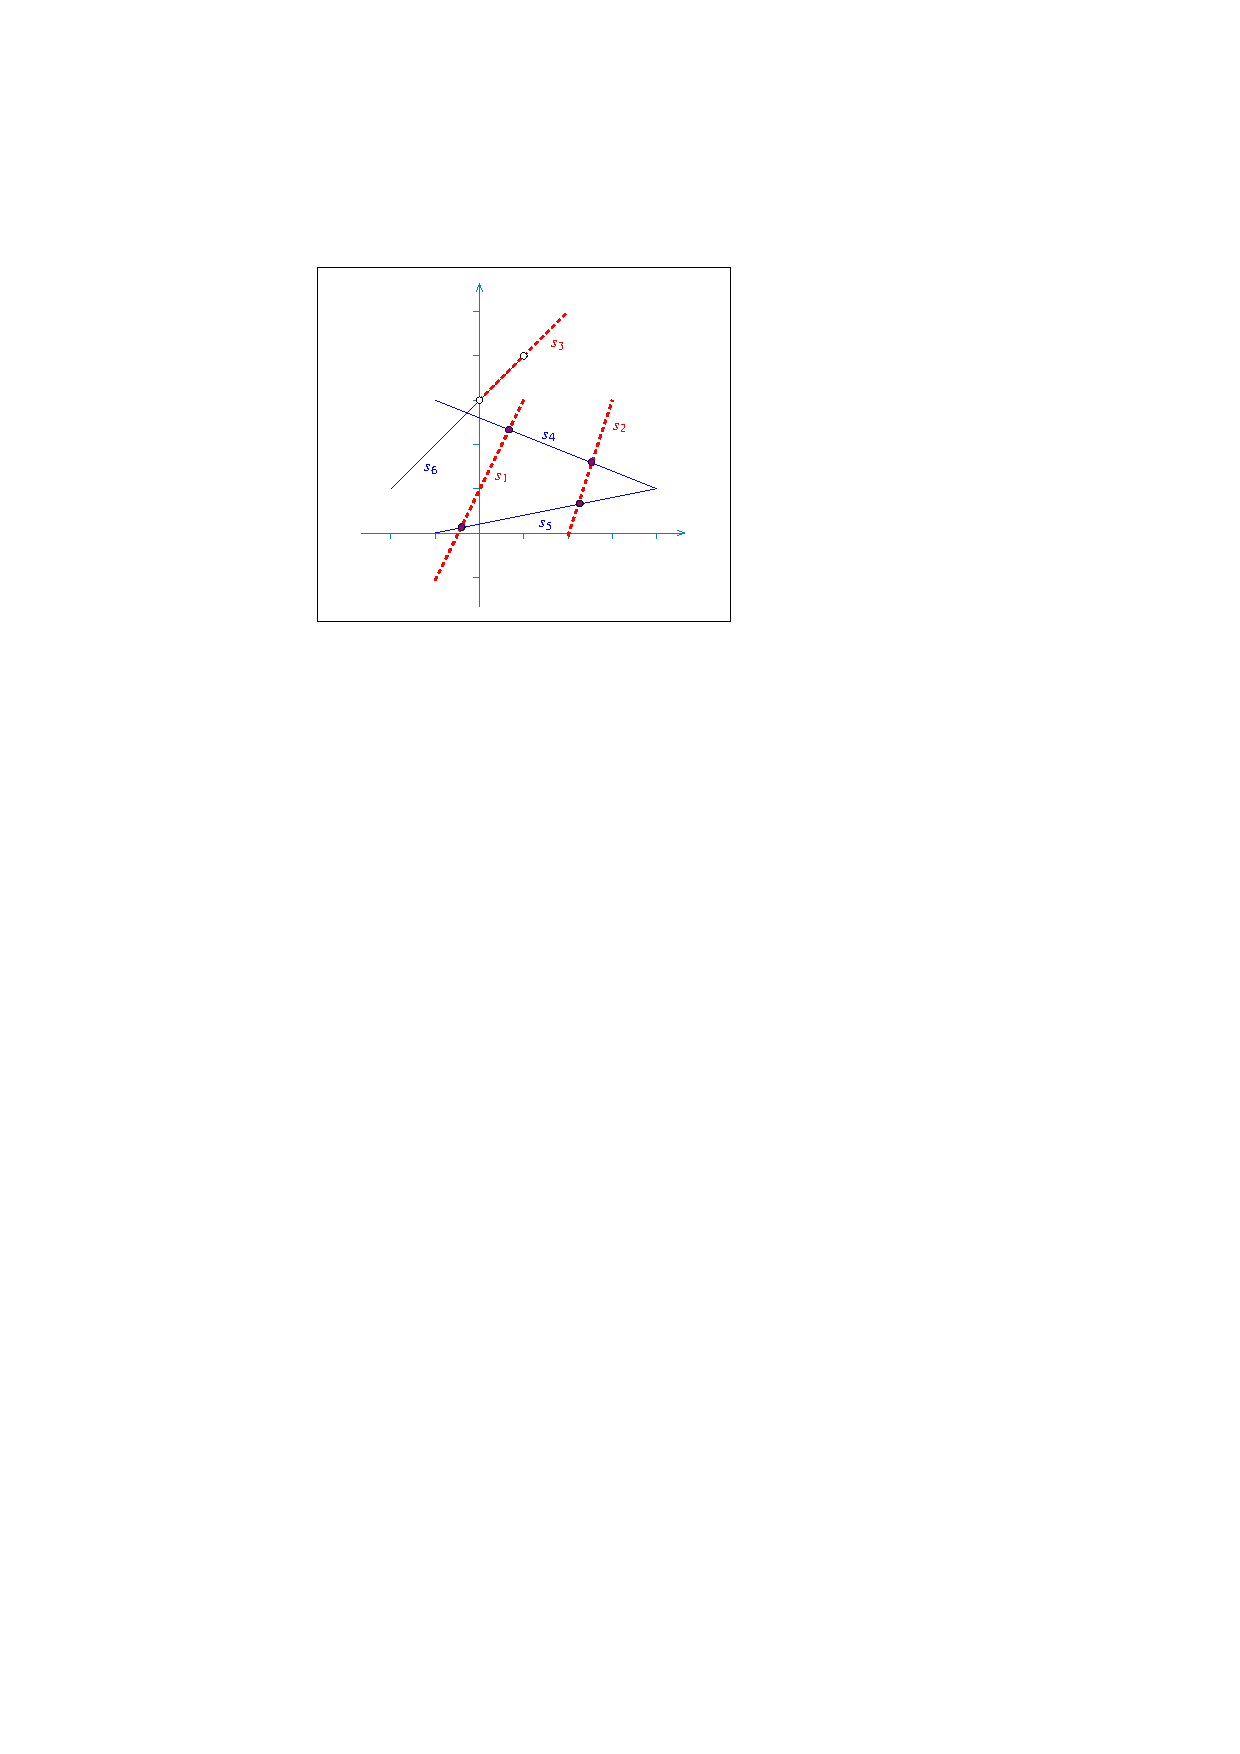
\includegraphics{Arrangement_on_surface_2/fig/ex_17}
  \end{center}
\end{ccTexOnly}
\begin{ccHtmlOnly}
  <p><center>
  <img src="./fig/ex_17.gif" border=0 alt="Example 17">
  </center>
\end{ccHtmlOnly}
\caption{An arrangement of six red and blue segments, as
constructed in \ccc{consolidated_curve_data.cpp}. Disks correspond to
red--blue intersection points, while circles mark the endpoints
of red--blue overlaps.\label{arr_fig:ex_17}}
\end{figure}

In the following example, we use \ccc{Arr_segment_traits_2} as our
base-traits class, attaching an additional {\em color} field to
the segments using the consolidated curve-data traits class. A
color may be either {\em blue} or {\em red}. Having constructed
the arrangement of colored segments, as depicted in
Figure~\ref{arr_fig:ex_17}, we detect the vertices that have incident 
edges mapped to both blue and red segments. Thus, they correspond
to red--blue intersection points. We also locate the edge that
corresponds to overlaps between red and blue line segments:

\ccIncludeExampleCode{Arrangement_on_surface_2/consolidated_curve_data.cpp}

\begin{figure}[t]
\begin{ccTexOnly}
  \begin{center}
  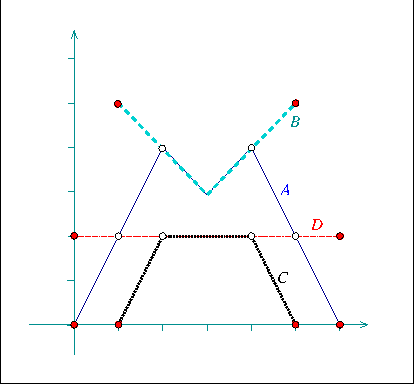
\includegraphics{Arrangement_on_surface_2/fig/ex_18}
  \end{center}
\end{ccTexOnly}
\begin{ccHtmlOnly}
  <p><center>
  <img src="./fig/ex_18.gif" border=0 alt="Example 18">
  </center>
\end{ccHtmlOnly}
\caption{An arrangement of four polylines, named A--D, as
constructed in \ccc{generic_curve_data.cpp}.\label{arr_fig:ex_18}}
\end{figure}

In the following example, we use \ccc{Arr_polyline_traits_2} as
our base-traits class, attaching an additional {\em name} field to
each polyline using the generic curve-data traits class. In case of
overlaps, we simply concatenate the names of the overlapping
polylines. Also notice how we replace the curve associated with
the edges that correspond to overlapping polylines with 
geometrically equivalent curves, but with a different data fields:

\ccIncludeExampleCode{Arrangement_on_surface_2/generic_curve_data.cpp}

The third example we give in this section is based on \ccc{dual_lines.cpp}
given in Section~\ref{arr_ssec:unb_global}. It constructs the arrangement
of the dual lines for a set of point given in an input file (by default we
use \ccc{coll_points.dat}, which contains $50$ points randomly selected
on the grid $[-100,100]\times[-100,100]$; the file contains two distinct
triplets of collinear points). Here we use the generic curve-data
decorator to attach the index of the primal point to each of the lines.
Doing so, we can go over the incident edges of each vertex whose degree is
greater than $4$ and report the subsets collinear points (if we have a vertex
of degree $d$, we actually need to go over $\frac{d}{2}$ edges, as each
incident line contributes exactly $2$ edges). Note that in this case the
dual line cannot overlap, so we use a dummy merge functor to instantiate
the curve-data traits:

\ccIncludeExampleCode{Arrangement_on_surface_2/dual_with_data.cpp}
